% ===========================================================================
%  Giant Killing in Football: An Information-Theoretic Analysis of Underdog
%  Upsets Using Causal Emergence
%
%  Sprint 6 draft manuscript (Introduction through Discussion).
%  Compile:  pdflatex manuscript && bibtex manuscript && pdflatex manuscript x2
% ===========================================================================
\documentclass[11pt,a4paper]{article}

\usepackage[margin=1in]{geometry}
\usepackage{amsmath,amssymb}
\usepackage{booktabs}
\usepackage{graphicx}
\usepackage{array}
\usepackage{caption}
\usepackage{subcaption}
\usepackage{float}
\usepackage{authblk}
\usepackage[hidelinks,breaklinks]{hyperref}
\usepackage[nameinlink]{cleveref}

\captionsetup{font=small,labelfont=bf}
\setlength{\parskip}{0.35em}
\setlength{\parindent}{0pt}

\newcommand{\code}[1]{\texttt{\small #1}}
\newcommand{\Vcom}{V_{\mathrm{CoM}}}
\newcommand{\Vdist}{V_{\mathrm{dist}}}
\newcommand{\Vcd}{V_{\mathrm{clust,dist}}}
\newcommand{\Vcv}{V_{\mathrm{clust,vel}}}

\title{\textbf{Giant Killing in Football:\\ An Information-Theoretic Analysis of
Underdog Upsets Using Causal Emergence}}
\author{Giant Killing Project}
\date{August 2026}

\begin{document}
\maketitle

% ===========================================================================
\begin{abstract}
\noindent
Underdog wins are a beloved part of any sport, and are a fundamental part of the history of soccer, where many giant killings take place with historic wins such as Senegal beating the World Cup reigning champions France in their first World Cup match ever in 2002, Greece winning the 2004 UEFA European Championship, and Leicester City winning the 2015/16 Premier League season.
  Even as these games are beloved by fans, statistically interpreting and predicting why and when an underdog team wins is generally opaque. 
  We test whether they carry a distinct emergent
coordination, defined by the causal-emergence coefficient $\Psi$ of Rosas
et al., 
  computed on tracking data reconstructed from StatsBomb 360 freeze frames for
136 matches (30 upsets, 106 rank-matched controls) across eight competition-seasons,
2020--2025. We extend on prior work on causal emergence in football in four ways through
non-parametric Kraskov--Stogbauer--Grassberger mutual-information estimation instead
of a Gaussian estimation, interaction of orders $\ell=1,2,3$ rather than $\ell=1$ alone, and
inter-team coupling metrics.

The results show that the level of $\Psi$ does not sufficiently determine underdog wins.
None of 54 pre-specified mixed-effects tests reached $p<0.05$ before correction, the
order profile does not differ by outcome ($p=0.995$ for the Match~Type $\times$ Order
interaction), the favourited team shows no measurable disruption, and a random forest on 260
trajectory features classifies upset versus control at chance (ROC-AUC $0.547$,
permutation $p=0.26$). However, the trajectory does seem to signal an underodg win.
  The slope over match
time of the underdog-minus-favourite emergence gap is positive in controls and negative
in upsets (Hedges' $g=-0.47$, permutation $p=0.024$, 6 of 18 feature $\times$ order cells
survive false-discovery-rate correction). Because negative $\Psi$ denotes
redundant, strictly organized play, this suggests that underdogs in giant killings become
progressively more structured relative to their opponents as the match develops.
  This is a temporal signature, and the opposite of the level-based prediction we set out to
test. 
  %This family was examined after the pre-specified tests returned null and is therefore exploratory.

We also show that the whole-minus-sum criterion is a poor instrument in this experiment,
and that its failure is specific to macro features that are linear aggregates of
the micro state. For those features $\Psi>0$ in $0.004\,\%$ of windows there is no indication for the hypothesised positive emergence, while for velocity-similarity clustering,
which is not a linear aggregate, $\Psi>0$ in $25.3\,\%$. Across the experiment $\Psi$ is almost
entirely determined by the micro sum ($r=0.995$), and $24\,\%$ of individual
mutual-information terms sit at the estimator's finite-sample ceiling of $2.57$ nats,
imposing a saturation floor. Minimum detectable effect at $80\,\%$ power is
$|g|\approx0.58$. We report the nulls, the one live effect,
and the measurement pathology together, and give concrete recommendations through a
$\Phi$ID-based synergy measure, non-linear macro features, longer windows, and a
pre-registered replication of the gap-trend endpoint.
\end{abstract}

\vspace{0.5em}
\noindent\textbf{Keywords:} causal emergence; partial information decomposition; football
analytics; underdog; collective behaviour; null results.

\newpage
\tableofcontents
\newpage

% ===========================================================================
\section{Introduction}
% ===========================================================================

Giant killings are some of the most celebrated events in football. Leicester City winning the Premier League after having been promoted from a league below, Senegal over France in 2002, Saudi Arabia over Argentina in 2022, and more recently with the 2026 World Cup in teams such as Cabo Verde.
These results are captivating because they defy expectation. 
Football is, on the available evidence, more pron to underdog wins, where across
twelve team ball sports, soccer has one of the highest empirical rates of a
historically weaker side beating a stronger one \cite{vicente2024}, a finding consistent
with earlier work on the parity and predictability of competitions \cite{benNaim2006}.

Yet the explanations offered are almost entirely post hoc and qualitative, unable to be expressed quantitatively, where
the underdog seems to have ``wanted it more'' or the giant became complacent or luck simply intervened. 
None are factually quantifiable explanations. 
A coach cannot train ``wanting it more'' into a team, and an analyst cannot quantify
complacency. The literature on quantitative football analytics has also not been able to predict underdog wins quantitatively either. 
Its dominant instruments rely on expected goals, possession, passing networks, physical output
which describe what a team did rather than how it organised itself to do it
\cite{low2020,buldu2018}. They are, moreover, largely reductive since they aggregate individual
contributions and therefore cannot in principle detect a team property that is not the
sum of its players.

Causal emergence helps to discover this discrepancy. Rosas et al.\ \cite{rosas2020},
building on partial information decomposition \cite{williams2010} and on earlier
accounts \cite{hoel2013,seth2010}, give a formal criterion for when a
macroscopic feature of a multivariate system carries predictive information about the
system's future that no individual part carries on its own. Applied to football, the
thus question becomes whether a team's collective configuration in its centre of mass, 
compactness, interaction network predicts its own future in a way that the
individual player positions do not? Cheng, Chang and Doya \cite{cheng2025} answered this
affirmatively for ordinary match dynamics, showing on 34 J-League matches that
average causal emergence over positional macro features correlates strongly with ball
possession ($R=0.74$--$0.79$) and rises for the attacking side in the sixty seconds before
a shot.

We seek to build on top of Cheng, Chand, and Doya by asking if giant killings reflect a genuine, transient surge of collective organisation in the weaker side,
then underdogs in upsets should show atypically high emergence, favourites should show
disrupted or collapsed emergence, or both. The intuition follows the idea that as the game progresses, favourites become complacent in defence and can allow a counterattack to become successful.
We set out to test this with four extensions
to \cite{cheng2025}, with a non-parametric mutual-information estimator that does not assume
joint Gaussianity, higher interaction orders, so that coordination localised in pairs or
triples of players such as a centre-back pairing, a midfield triangle and can be distinguished
from team-wide coordination, explicit inter-team coupling, so that disruption of the
favourite can be measured rather than inferred, and a pre-specified analysis plan with
matched controls, correction for multiplicity, and a sensitivity battery.

% What we found
We found that the level-based hypothesis fails under
every robustness variant we examined. What survives is a temporal effect that runs
opposite to the direction we predicted. Relative to the favorites, underdogs in upsets
become progressively more redundancy-dominated, more drilled, and less synergistic
as the match proceeds, while in control matches the reverse holds. Underneath both
results sits a measurement problem we did not anticipate and that we regard as the most
transferable contribution of this paper. The whole-minus-sum criterion $\Psi$, evaluated
on 60-second windows of football tracking data, is dominated by definitional redundancy
and is estimator-saturated over a large fraction of its range. 

\paragraph{Contributions.} (i) The first application of causal emergence to match
outcomes rather than in-match phases on a list of upsets and
controls. (ii) A null $\Psi$ level that does not distinguish
giant killings, at any order, for any macro feature, under any sensitivity variant, and
does not support classification above chance. (iii) One exploratory positive result which is the
emergence gap trend. (iv) An explanation of
why the whole-minus-sum criterion is the wrong instrument, with quantitative
evidence via the redundancy decomposition and the estimator ceiling, and specific
alternatives. (v) A complete, open replication package.

\Cref{sec:background} sets out the theoretical framework. \Cref{sec:methods} describes the
dataset, the tracking reconstruction, the estimator and the analysis plan.
\Cref{sec:results} reports results by research question. \Cref{sec:discussion} interprets
them, draws out the practical implications, and states what would settle the question.

% ===========================================================================
\section{Background}
\label{sec:background}
% ===========================================================================

\subsection{Causal emergence}

Consider a system of $n$ parts observed at times $t$ and $t'>t$, with micro state
$X_t=(X^1_t,\dots,X^n_t)$, and a resulting feature $V_t$ that adds no
predictive power over $X_{t'}$ once $X_t$ is known exactly, so that $V_t-X_t-X_{t'}$ is a
Markov chain. Rosas et al.\ \cite{rosas2020} define $V_t$ to exhibit causal emergence of
order $k$ when its unique information about the future is positive in the partial information decomposition sense.
\begin{equation}
\mathrm{Un}^{(k)}(V_t; X_{t'} \mid X_t) > 0 .
\label{eq:def}
\end{equation}
Computing \eqref{eq:def} requires a choice of PID functional and is generally intractable. 
Rosas et al.\ therefore supply a practical sufficient criterion that
depends only on pairwise mutual informations
\begin{equation}
\Psi^{(k)}_{t,t'}(V) \;:=\; I(V_t;V_{t'}) \;-\; \sum_{|\alpha|=k} I\!\left(X^\alpha_t; V_{t'}\right)
\label{eq:psi}
\end{equation}
where $\alpha$ ranges over subsets of parts of size $k$ and $X^\alpha_t$ is their joint
state. $\Psi^{(k)}>0$ is sufficient but not necessary for causal emergence.

The interpretation used throughout this paper follows \cite{rosas2020,cheng2025}.
$\Psi>0$ is synergy-dominated where the collective carries predictive information that the
parts do not. $\Psi<0$ is redundancy-dominated where the parts, taken together, predict the
macro future better than the macro state does, which is the signature of synchronised,
mutually predictable, well-drilled behaviour. Rosas et al.\ are explicit that
\eqref{eq:psi} belongs to the whole-minus-sum family and therefore double-counts
redundancy across all $n$ marginals, so that redundancy drives $\Psi$ negative and a
negative value is inconclusive rather than evidence of absence. This caveat, stated in
their \S III\,A, turns out to govern our results so we return to it in
\cref{sec:res-measure}.

\subsection{Causal emergence in football}

Cheng et al.\ \cite{cheng2025} instantiate this framework on football tracking data using
four macroscopic features via the team centre of mass $\Vcom$, the mean distance of players
to the field centre $\Vdist$, and two weighted clustering coefficients on the player
interaction graph, one with edge weight $w_{uv}=1/d_{uv}$ (inverse distance, $\Vcd$) and
one with $w_{uv}=S_uS_v(\cos\Delta\theta+1)$ (velocity similarity, $\Vcv$), computed with
the Onnela definition \cite{onnela2005}. Their micro features are the corresponding
per-player quantities. Restricting to $\ell=1$ and estimating mutual information with a
Gaussian plug-in, they find that match-average $\Psi$ on $\Vdist$ and $\Vcom$ correlates
strongly with the home--away possession differential ($R=0.79$ and $0.74$), that $\Vcd$
correlates moderately ($R=0.58$), and that $\Vcv$ does not ($R=0.06$). In the sixty
seconds before a shot, the attacking team's $\Psi$ rises and the defending team's falls.

Two features of that design matter for ours. First, their tracking data are proprietary
25\,Hz optical recordings, down-sampled to 1\,Hz which are accurately complete and detailed.
Second, their analysis falls within matches because it compares phases and roles, not outcomes across matches. 
Both differences bear directly on our results.

\subsection{Upsets}

Existing quantitative work on upsets is largely descriptive and event-based. Analyses of
World Cup upsets find that winning underdogs concede possession, passing accuracy and
touches while producing more shots on target, clearances and aerial duels.
%--- a direct, counter-attacking, defensively disciplined profile. 
Vicente et al.\
\cite{vicente2024} approach the phenomenon structurally, ranking sports by an underdog
achievement score and attributing football's high score to randomness factors intrinsic to
the game (goal size relative to the number of defenders, low scoring frequency, ball
handling). Wunderlich et al.\ \cite{wunderlich2021} show that the randomness contribution
to goal scoring decreases as a match progresses, which disadvantages weaker teams.

None of this literature addresses collective organisation. Our question is whether the
tactical profile the event data describe has an information-theoretic correlate at the
level of team structure.

\subsection{Research questions}

\begin{description}
\item[RQ1 (Emergence signatures).] Do giant killings show different $\Psi$ from expected
results such as underdogs higher, favourites lower?
\item[RQ2 (Order).] At what interaction order does any such effect manifest: team-wide
($\ell=1$), pairs ($\ell=2$), or triples ($\ell=3$)?
\item[RQ3 (Temporal dynamics).] Does underdog emergence build gradually or in bursts? Is
there a tipping point at which the underdog's $\Psi$ overtakes the favourite's?
\item[RQ4 (Disruption).] Can we quantify the underdog disrupting the favourite's
coordination?
\item[RQ5 (Spatial signatures).] Which macro features, if any, discriminate giant
killings?
\end{description}

We additionally defined three summary metrics: the Emergence Asymmetry Index
$\mathrm{EAI}=(\Psi_u-\Psi_f)/(\Psi_u+\Psi_f+\epsilon)$, the Disruption Coefficient
$\mathrm{DC}=I(V_u;V_f)/H(V_f)$, and the Synergy--Redundancy Ratio
$\mathrm{SRR}=\max(0,\Psi)/(|\min(0,\Psi)|+\epsilon)$. All three decline on continuous
football data, and \cref{sec:metrics} documents the failure modes and the stabilised
replacements we use.

% ===========================================================================
\section{Data and methods}
\label{sec:methods}
% ===========================================================================

\subsection{Data}
\label{sec:corpus}

\paragraph{Upset definition.} A match is a candidate giant killing when the pre-match
mismatch is large and the weaker side wins. We compute a continuous upset score in
$[0,1]$ from five normalised pre-match gaps which are rolling Elo including a 70-point home
advantage (weight $0.40$), log squad-value ratio from Transfermarkt ($0.25$), form
differential over the previous ten matches ($0.20$), pre-match expected-goals differential
from Understat ($0.10$), and a manager-tenure proxy ($0.05$), all multiplied by $1.0$ if
the underdog won, $0.5$ for a draw and $0.0$ for a loss, and thresholded at $0.65$. The
threshold was set so that roughly $10\,\%$ of fixtures in a typical top-five league season
are flagged, matching the empirical shock-result frequency.

\paragraph{Controls.} For each flagged upset we retain rank matched fixtures meeting the
same mismatch criteria in which the favourite won as expected. This yields a
matched-mismatch design where every match in the dataset, upset or control, is a
fixture with a large paper gap. This is deliberate and it has a consequence we flag now
and return to in \cref{sec:res-rq4} since the dataset contains no even-game layer, so a
general losing effect cannot be separated from a giant-killing specific one.

\paragraph{Dataset.} Intersecting the upset and control lists with matches for
which StatsBomb 360 freeze frames are available \cite{statsbomb} gives 136
matches: 30 upsets and 106 controls, spanning 2020-10-17 to 2025-07-22
(\cref{tab:corpus}). The dataset is dominated by international tournaments, which is a
generalisability limitation: club football, and in particular the cup competitions where
giant killings are most frequent, is barely represented, only having matches from specific teams and seasons such as Barcelona 20/21 league matches and Bayer Leverkusen 23/24 league matches.

\begin{table}[H]
\centering
\small
\begin{tabular}{@{}lrrl@{}}
\toprule
\textbf{Competition} & \textbf{Matches} & \textbf{Upsets} & \textbf{Window} \\
\midrule
FIFA World Cup 2022        & 40 & 11 & Nov--Dec 2022 \\
FIFA Women's World Cup 2023& 37 &  8 & Jul--Aug 2023 \\
UEFA Euro 2024             & 24 &  6 & Jun--Jul 2024 \\
UEFA Women's Euro 2022     & 12 &  1 & Jul 2022 \\
UEFA Women's Euro 2025     & 10 &  2 & Jul 2025 \\
UEFA Euro 2020             &  7 &  1 & Jun 2021 \\
Bundesliga 2023/24         &  3 &  0 & Oct 2023--May 2024 \\
La Liga 2020/21            &  3 &  1 & Oct 2020--Feb 2021 \\
\midrule
\textbf{Total}             & \textbf{136} & \textbf{30} & 2020-10-17 -- 2025-07-22 \\
\bottomrule
\end{tabular}
\caption{Upsets and controls. The design is matched-mismatch. Controls are fixtures with the
same pre-match gap in which the favourite won.}
\label{tab:corpus}
\end{table}

\subsection{Tracking reconstruction}

StatsBomb 360 provides a freeze frame of visible player positions at each on-ball event, roughly one frame every 1.9\,s, concentrated near the ball, with off-camera players
absent. We reconstruct continuous 1\,Hz trajectories following Penn et al.\
\cite{penn2023} utilizing an ARMAX one-step predictor for player position with the ball position as
exogenous input, Hungarian assignment of observed positions to trajectories under that
predictive model, and velocity-corrected interpolation between observed points, in which
the linear interpolant is corrected by the time integral of the visible mean team velocity
scaled by $\alpha\approx0.5$.

Penn et al.\ report a mean error of $7.33$\,m for off-camera players on held-out data,
against $3.45$\,m overall. The LSTM--GNN imputer of Everett et al.\ \cite{everett2023}
achieves $\sim6.9$\,m from event data alone and is the natural cross-validation benchmark;
we did not run it, and this remains the most important unaddressed check on our input
data. Reconstruction error is symmetric and partially averages out over a 60\,s window,
but it is not innocuous for the clustering coefficients, which are non-linear in the
pairwise distances.

For preprocessing, positions are resampled to a 1\,Hz grid; velocities are finite
differences; goalkeepers are dropped and each team is truncated at its first red card, so
that all analyses use exactly ten outfielders per side, following \cite{cheng2025}. The
tracking clock is aligned to the event clock as
$t=(\text{period}-1)\cdot2700+60\cdot\text{minute}+\text{second}$. Windows are $60$\,s
long and advance in $10$\,s steps.

\subsection{Features}

Six macro features are computed per team per window: the four of \cite{cheng2025} plus two
composites.

\begin{table}[H]
\centering
\small
\begin{tabular}{@{}llp{7.6cm}@{}}
\toprule
\textbf{Name} & \textbf{Dim} & \textbf{Definition} \\
\midrule
\code{V\_com}   & 2 & centre of mass, $\tfrac1P\sum_i(x_i,y_i)$ \\
\code{V\_dist}  & 1 & mean distance to pitch centre, $\tfrac1P\sum_i\lVert p_i-(60,40)\rVert$ \\
\code{V\_cdist} & 1 & Onnela weighted clustering coefficient, $w_{uv}=1/d_{uv}$ \\
\code{V\_cvel}  & 1 & Onnela weighted clustering coefficient, $w_{uv}=S_uS_v(\cos\Delta\theta+1)$ \\
\code{V\_all}   & 5 & all four jointly \\
\code{V\_fast}  & 3 & \code{V\_com} $+$ \code{V\_dist} \\
\bottomrule
\end{tabular}
\caption{Macroscopic features. \code{V\_com} and \code{V\_dist} are linear aggregates of the micro state, the clustering coefficients are not.}
\label{tab:features}
\end{table}

Micro features are the $2P=20$ individual coordinates. At $\ell=1$ the sum in
\eqref{eq:psi} has $10$ terms, at $\ell=2$ it has $\binom{10}{2}=45$, and at $\ell=3$ it
has $\binom{10}{3}=120$. At $\ell=3$ we retain only triples whose members are pairwise
within $25$\,m of one another in mean window position, capped at $60$ triples, and rescale
the sum by $n_{\text{total}}/n_{\text{selected}}$. This Horvitz--Thompson-style correction
assumes the retained triples are representative, which proximity selection deliberately
violates. Both the scaled and unscaled sums are emitted, and the induced bias is measured
against the exhaustive sum.

\subsection{Estimation}

All information quantities use the Kraskov--St\"ogbauer--Grassberger estimator \#1
\cite{kraskov2004}. For samples $\{(x_i,y_i)\}_{i=1}^N$ and neighbour count $k$, with
$\epsilon_i$ twice the distance to the $k$th nearest neighbour in the joint space under
the Chebyshev norm and $n^{(i)}_x,n^{(i)}_y$ the marginal counts within $\epsilon_i$,
\begin{equation}
\hat I(X;Y)=\psi(k)-\frac1N\sum_{i=1}^{N}\!\left[\psi\!\left(n^{(i)}_x+1\right)+\psi\!\left(n^{(i)}_y+1\right)\right]+\psi(N).
\label{eq:ksg}
\end{equation}
Differential entropies for the Disruption Coefficient use the Kozachenko--Leonenko
estimator \cite{kozachenko1987}. Production runs use $k=4$; $k\in\{3,4,7,10\}$ is varied
in sensitivity analysis.

\Cref{eq:ksg} was validated against the closed form for a bivariate Gaussian,
$I=-\tfrac12\ln(1-\rho^2)$, with absolute error below $10^{-2}$ nats at $N=4000$, $k=4$
across $\rho\in\{0,0.3,0.6,0.9\}$, and the entropy estimator against
$\tfrac{d}{2}\log(2\pi e)$ for $d\in\{1,2,3,5\}$. An $O(N^2)$ transcription test and the
$k$-d-tree implementation agree with the implementation.

Three estimator defects, are found and corrected. These are reported because each
would have produced a plausible-looking but wrong result. (i) Ties produced
infinities. Because the 1\,Hz grid interpolates linearly between sparse events, the
velocity-derived $\Vcv$ is piecewise constant over long runs with an absolute neighbour
tolerance those runs give $\epsilon_i=0$, a neighbour count of $-1$, and $\psi(0)=-\infty$.
The fix is a relative tolerance, clamping of counts at zero, and tie-breaking jitter of
$10^{-10}$ in standardised units, as Kraskov et al.\ recommend. 
(ii) Chebyshev scale
dominance. KSG uses the max norm so a joint feature vector is governed by whichever
dimension has the largest numerical spread. Raw macro features span
$\sigma(\Vcom)\approx19$\,m against $\sigma(\Vcd)\approx0.10$; left unstandardised, the
five-dimensional \code{V\_all} returned numerically identical $\Psi$ to the
three-dimensional \code{V\_fast}, the clustering dimensions contributing nothing. All
estimates therefore use per-window $z$-scored inputs with $V_t$ and $V_{t'}$ sharing one
scaler. Mutual information is invariant to this transform in theory; the estimator is not.
(iii) Cost. Per-subset tree builds are pure overhead at $N\approx59$; the micro-side
distances do not depend on the macro feature. Precomputing the $2P$ per-coordinate distance
matrices once per window and forming subset distances by elementwise maximum gives
bit-identical results at a fraction of the cost.

\subsection{The three proposed metrics, and their stabilised forms}
\label{sec:metrics}

Each metric is emitted exactly as specified and in a repaired form, because all
three degenerate here.

\textbf{EAI.} $(\Psi_u-\Psi_f)/(\Psi_u+\Psi_f+\epsilon)$ is bounded in $[-1,1]$ only when
both $\Psi$ are non-negative. Empirically $\Psi<0$ almost everywhere so the denominator is
a sum of two same sign large numbers that pass through zero exactly when the teams are
comparable which is where the hypothesis locates the interesting behaviour. The
stabilised form uses $|\Psi_u|+|\Psi_f|+\epsilon$ and is bounded, same sign, same monotonicity,
and no pole.

\textbf{DC.} $I(V_u;V_f)/H(V_f)$ divides by a differential entropy which is
scale-dependent and here routinely negative ($\approx-5$ nats), negating the ``fraction of entropy explained'' explanation. 
We store $I(V_u;V_f)$ and
$H(V_f)$ separately and report the informational coefficient of correlation
$\mathrm{dc}_{ic}=1-e^{-2I}$, bounded in $[0,1)$ and invariant to smooth
reparameterisation of $V$.

\textbf{SRR.} $\max(0,\Psi)/(|\min(0,\Psi)|+\epsilon)$ evaluated at a single $\Psi$
collapses to $0$ or to $\Psi/\epsilon\approx10^9$ and is a ratio statistic requiring a
set of values. Per-window, rolling-block and whole-match versions are emitted. On
the linear macro features $\Psi$ is essentially never positive, so match-level SRR is
zero or near-zero throughout and is itself a finding (\cref{sec:res-measure}).

\subsection{Analysis plan}
\label{sec:plan}

We implement window thinning where $\Psi$ is emitted every 10\,s from a 60\,s window so
that consecutive records share 50 of 60 seconds. All models therefore use
non-overlapping windows only ($\text{window\_start}\bmod 60=0$), retaining
$231{,}492$ of $1{,}384{,}566$ records ($16.7\,\%$), with residual within-match dependence
absorbed by a random intercept.

For the variance structure, the intraclass correlation of $\Psi$ is between $0.004$
and $0.014$ depending on macro feature. 98--99\,\% of the variance is
window to window within a single match. A
between-group difference of $\sim0.2$ nats sits inside a within-match standard deviation
of $\sim3.2$ nats, which is why pooled dataset medians appear identical between groups and
why the random intercept is mandatory rather than decorative.

For the model, RQ1 fits, for all 6 macro features $\times$ 3 orders,
\begin{equation}
\Psi_{ijt}=\beta_0+\beta_1\text{Upset}_{ij}+\beta_2\text{Time}_t+\beta_3(\text{Upset}\times\text{Time})_{ijt}
+\beta_4\text{Role}_{ij}+\beta_5(\text{Upset}\times\text{Role})_{ij}+u_i+\epsilon_{ijt},
\label{eq:rq1}
\end{equation}
with $u_i\sim\mathcal N(0,\sigma_u^2)$ a per-match random intercept and time and role
centred, so $\beta_1$ estimates the average upset effect rather than its value at kickoff
for the favourite. Coefficients are reported as $\beta_1/\hat\sigma_u$ to permit comparison
across orders, since $|\Psi|$ scales mechanically with the number of subsets. All 54 tests
form one family under Benjamini--Hochberg \cite{benjamini1995}. Because upsets end with the
underdog ahead by construction, goal times were extracted from the event feed (405 goals
across 136 matches), each window carries the goal difference at its start, and every RQ1
model is refitted with that covariate.

RQ2 is Order (3, within) $\times$ Match Type (2, between) $\times$ Role (2, within), match
as subject, fitted as a linear mixed model so sphericity need not be assumed, with
Greenhouse--Geisser-corrected $F$-tests reported alongside. $\Psi$ is $z$-scored
within order before testing, otherwise the Order main effect is reflecting only that $120>45>10$ subsets are being summed. RQ3 compares mean
$\Psi$ curves on a normalised-time grid by permutation over whole match labels, locates
change points in the gap $g(t)=\Psi_{\text{und}}(t)-\Psi_{\text{fav}}(t)$ by binary
segmentation with an $L_2$ cost \cite{killick2012}, and compares per-match least-squares
slopes of $g(t)$. RQ4 fits favourite-only models and the disruption coefficient. RQ5 trains
a random forest on 260 match-level trajectory summaries with stratified 5-fold
cross-validation, class-weight balancing, a 200-draw permutation null in which the whole
CV pipeline is re-run on shuffled labels, and temporal blocking.

In determining sensitivity, alternative upset definitions (rank gap $\ge0,10,20,30$), MAD
outlier exclusion, effective-sample thresholds, excluding the first and last $10\,\%$ of
each match, window lengths $W\in\{30,60,90\}$\,s and $k\in\{3,4,7,10\}$ recomputed from
scratch on a 60-match subsample, a 324-cell specification curve \cite{simonsohn2020} over
\{summary statistic\} $\times$ \{windowing\} $\times$ \{feature\} $\times$ \{order\}
$\times$ \{role\}, and a placebo calibration repeating the entire specification curve on 25
label shuffles.

We deviated from the plan slightly since (i) The proposal targeted
50--75 upsets and the 360 dataset delivered 30, (ii) RQ4's third condition that the favourite loses
to an equally strong opponent does not exist in a matched-mismatch dataset and was not
tested, and (iii) The gap trend family analysed in \cref{sec:res-rq3} was examined
after the pre-specified tests returned null. It is exploratory and is reported as
such.

% ===========================================================================
\section{Results}
\label{sec:results}
% ===========================================================================

The production run processed all 136 matches, producing $1{,}384{,}566$ window-level
records over $116{,}709$ distinct windows, with $99.98\,\%$ of estimates computed
successfully and a median of 59 usable frames per 60\,s window. Reconciliation against an
independent earlier implementation is accurate on $9{,}371$ audited windows in which the recomputed
coefficient matches the stored value to $0.0$ nats.

\subsection{The measure behaves pathologically before any hypothesis is tested}
\label{sec:res-measure}

$\Psi$ is negative in $95.5\,\%$ of windows, and this is structural rather than empirical
(\cref{fig:floor}a). Across the dataset, the micro sum averages $12.3$ nats against $1.4$
for the macro term, a factor of $8.5$, so that $\Psi\approx-\sum_i I(X^i_t;V_{t'})$
with $\mathrm{corr}(\Psi,-\sum_i I)=0.9996$ (\cref{fig:floor}b). Two mechanisms produce
this. First, whole-minus-sum measures double-count redundancy across all $n$ marginals, as
Rosas et al.\ note \cite{rosas2020}. Second, $\Vcom$ is the mean of the micro
positions, so every player is mechanically informative about it, in every match and
every team, regardless of tactics.

Moreover, the degeneracy is confined to macro features that are linear
aggregates of the micro state (\cref{tab:headroom}). For $\Vcom$, $\Vdist$,
\code{V\_fast} and \code{V\_all}, $\Psi$ exceeds zero in $0.004\,\%$ of windows pooled and
in no window at all for \code{V\_fast}. The Synergy--Redundancy Ratio, defined as a
ratio of positive to negative parts, is correspondingly zero for all 136 matches on
\code{V\_fast} and for all but a handful on the others. For the two clustering
coefficients, which are not linear in the micro state, the picture is different: $\Psi>0$
in $2.0\,\%$ of windows for $\Vcd$ and $25.3\,\%$ for $\Vcv$, and match-level SRR is
non-zero in all 136 matches for both, though still small in absolute terms
($\max=0.14$), so even these features remain redundancy-dominated. The same ordering shows
up in the medians where $|\Psi|$ is largest for the linear aggregates ($\Vcom$: $-15.4$,
\code{V\_fast}: $-14.1$) and smallest for the clustering coefficients ($\Vcv$: $-2.4$,
$\Vcd$: $-5.3$).

\begin{table}[H]
\centering
\small
\begin{tabular}{@{}lrrrr@{}}
\toprule
\textbf{Macro feature} & \textbf{linear?} & \textbf{median $\Psi^{(1)}$} & \textbf{\% windows $\Psi>0$} & \textbf{matches with SRR $>0$} \\
\midrule
\code{V\_com}   & yes & $-15.39$ & $0.003$  & 2 / 136 \\
\code{V\_fast}  & yes & $-14.10$ & $0.000$  & 0 / 136 \\
\code{V\_all}   & mixed & $-10.52$ & $0.005$ & 7 / 136 \\
\code{V\_dist}  & yes & $-9.20$  & $0.008$  & 8 / 136 \\
\code{V\_cdist} & no & $-5.33$  & $1.99$ & 136 / 136 \\
\code{V\_cvel}  & no & $-2.42$  & $25.26$ & 136 / 136 \\
\bottomrule
\end{tabular}
\caption{Headroom for positive emergence, by macro feature, over the 231{,}492
non-overlapping analysis windows. Where the macro feature is a linear aggregate of the
micro state, the criterion has effectively no positive range, and where it is not, it does.}
\label{tab:headroom}
\end{table}

At $N\approx59$ samples per window and $k=4$, the KSG estimator has a finite sample ceiling where no per-player
term exceeds $2.5652$ nats, and $24\,\%$ of all per-player mutual-information terms
sit at that ceiling (\cref{fig:floor}c). Because $\Psi^{(1)}=I_{\text{macro}}-\sum_i I$,
ten saturated terms impose a floor at $\Psi\approx-23.1$ nats, and 29--34\,\% of window-level
$\Psi$ values for $\Vcom$, $\Vdist$ and \code{V\_fast} lie below $-23$ nats. Over a substantial share of its
range, therefore, $\Psi$ is not measuring team coordination and instead reports that
the estimator has run out of dynamic range. Longer windows are the obvious remedy and are
partially explored in \cref{sec:res-sens}.

The consequence for the hypothesis is immediate. We predicted that underdogs would show
positive emergence in bursts. On the four macro features that dominate the analysis
by magnitude, and on which \cite{cheng2025} reported its strongest results, there is
no headroom in which such bursts could be observed at all. 
The prediction is not so much refuted as untestable with this instrument on these features.

\begin{figure}[H]
\centering
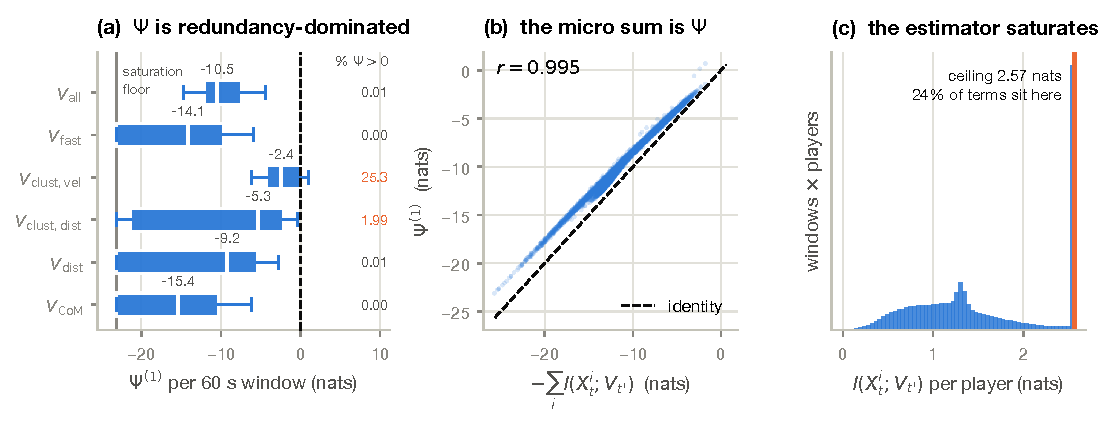
\includegraphics[width=\textwidth]{figures/fig1_redundancy_floor.pdf}
\caption{The criterion is dominated by redundancy and is estimator-saturated.
(a) Distribution of $\Psi^{(1)}$ per 60\,s window by macro feature (box: quartiles,
whiskers: 5th--95th percentile, annotation: median, right column: percentage of windows
with $\Psi>0$). $|\Psi|$ is largest, and positive range scarcest, for the linear
aggregates, the two non-linear clustering coefficients are the only features with usable
headroom. The grey line marks the saturation floor at $-23.1$ nats.
(b) $\Psi$ against the negated micro sum for \code{V\_all} (6{,}000-window sample),
$r=0.995$. The vertical offset from the identity line is $I(V_t;V_{t'})$, the entire macro
contribution. (c) Distribution of the per-player term $I(X^i_t;V_{t'})$ for the linear
features: $24\,\%$ of terms sit at the estimator's ceiling of $2.57$ nats at $N\approx59$,
$k=4$.}
\label{fig:floor}
\end{figure}

\subsection{RQ1 --- the level of \texorpdfstring{$\Psi$}{Psi} carries no outcome signal}
\label{sec:res-rq1}

\textbf{Null.} Zero of 54 coefficient tests from \eqref{eq:rq1} reach $p<0.05$ before
correction (\cref{fig:rq1}); the joint likelihood-ratio test dropping all upset terms is
non-significant for every feature--order pair (smallest $p=0.18$, all $p_{\text{FDR}}=0.95$).
Adjusting for goal difference does not change this. The largest standardised effect
anywhere is $\Vcv$ at $\ell=1$ ($\beta_1/\hat\sigma_u=-0.43$, $p=0.081$) --- notably, the
one macro feature that is not an average of its micro inputs.

\begin{figure}[H]
\centering
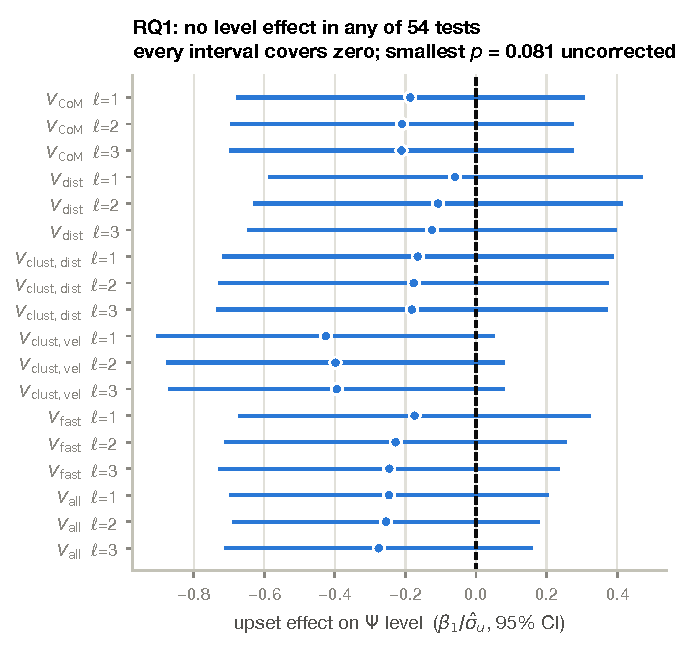
\includegraphics[width=0.62\textwidth]{figures/fig2_rq1_forest.pdf}
\caption{\textbf{RQ1 is null.} Standardised upset effect on the level of $\Psi$ from the
pre-specified mixed model \eqref{eq:rq1}, for each macro feature $\times$ interaction
order, with 95\,\% confidence intervals. Every interval covers zero. The most negative
point estimate is $\Vcv$ at $\ell=1$.}
\label{fig:rq1}
\end{figure}

\subsection{RQ2 --- no order-specific signature}

\textbf{Null.} The RQ2 question is the Match Type $\times$ Order interaction, at
$\chi^2=0.010$, $p=0.995$, partial $\eta^2<0.001$. There is no evidence that upset
emergence manifests preferentially at pair or triple level. The Match Type main effect is
also null ($p=0.188$). The only significant term is the Role main effect
($\chi^2=24.09$, $p<10^{-6}$, partial $\eta^2=0.029$), which merely restates that
underdogs and favourites differ is true by construction in a mismatch dataset. That the
Order main effect is non-significant ($p=0.844$) confirms the within-order standardisation
removed the mechanical scaling as intended. Per-cell repeated-measures ANOVAs with
Greenhouse--Geisser correction agree (all $p_{\text{GG}}>0.34$; largest partial $\eta^2=0.031$,
upset underdogs).

The methodological extension to $\ell=2,3$ --- one of the four ways this work was to
improve on \cite{cheng2025} --- therefore bought no additional discrimination. Whether
that is a fact about football or about the criterion (\cref{sec:res-measure}) cannot be
settled from these data.

\subsection{RQ3 --- levels are null but gap trend is not}
\label{sec:res-rq3}

\paragraph{Levels and tipping points are null.} Mean $\Psi$ curves on a normalised-time grid
are indistinguishable between groups under permutation over whole match labels
(preserving within-match autocorrelation), for both $\sup_t|\Delta(t)|$ and $\int\Delta^2$
statistics; nothing survives correction (smallest $p_{\text{FDR}}=0.54$). Neither the
change-point location in $g(t)$ ($p=0.76$), nor the first zero-crossing ($p=0.27$), nor the
fraction of the match with $g>0$ ($p=0.50$) separates the groups. In most matches $g$ never
crosses zero at all, so there is no tipping point to predict. 
%%%%%%%%%%%%%%%%%%%%%
The RQ3 hypothesis as originally posed is not merely unsupported but inapplicable.
%%%%%%%%%%%%%%%%%%%%%


\paragraph{Effects in the gap trend.} Fitting a least-squares line to $g(t)$ over
normalised match time and comparing per-match slopes between groups gives the one live
result in this study (\cref{fig:gap}, \cref{fig:traj}, \cref{tab:gaptrend}). Nine of 18
feature--order cells are significant raw and six survive Benjamini--Hochberg, with
$|g|$ from $0.34$ to $0.62$ at or above the dataset minimum detectable effect. Control
slopes are positive in all 18 cells. A permutation test on the primary
specification (\code{V\_all}, $\ell=1$, 20{,}000 draws shuffling whole match labels) gives
an observed slope difference of $-0.489$ nats per match, $p=0.024$.

\begin{table}[H]
\centering
\small
\begin{tabular}{@{}llrrrrr@{}}
\toprule
Feature & Order & upset slope & control slope & $g$ & $p$ & $p_{\text{FDR}}$ \\
\midrule
\code{V\_all}   & 3 & $-3.706$ & $+4.678$ & $-0.560$ & $0.0001$ & $0.0015$ \\
\code{V\_all}   & 2 & $-1.311$ & $+1.677$ & $-0.550$ & $0.0002$ & $0.0015$ \\
\code{V\_fast}  & 3 & $-1.916$ & $+4.797$ & $-0.383$ & $0.0009$ & $0.0056$ \\
\code{V\_all}   & 1 & $-0.207$ & $+0.282$ & $-0.468$ & $0.0046$ & $0.0175$ \\
\code{V\_fast}  & 2 & $-0.432$ & $+1.734$ & $-0.340$ & $0.0049$ & $0.0175$ \\
\code{V\_cdist} & 2 & $-2.418$ & $+1.330$ & $-0.624$ & $0.0117$ & $0.0350$ \\
\bottomrule
\end{tabular}
\caption{The six feature--order cells surviving FDR correction on the gap-slope comparison.
Slopes are in nats per normalised match. Control slopes are positive in all 18 cells,
including the twelve not shown.}
\label{tab:gaptrend}
\end{table}

\begin{figure}[H]
\centering
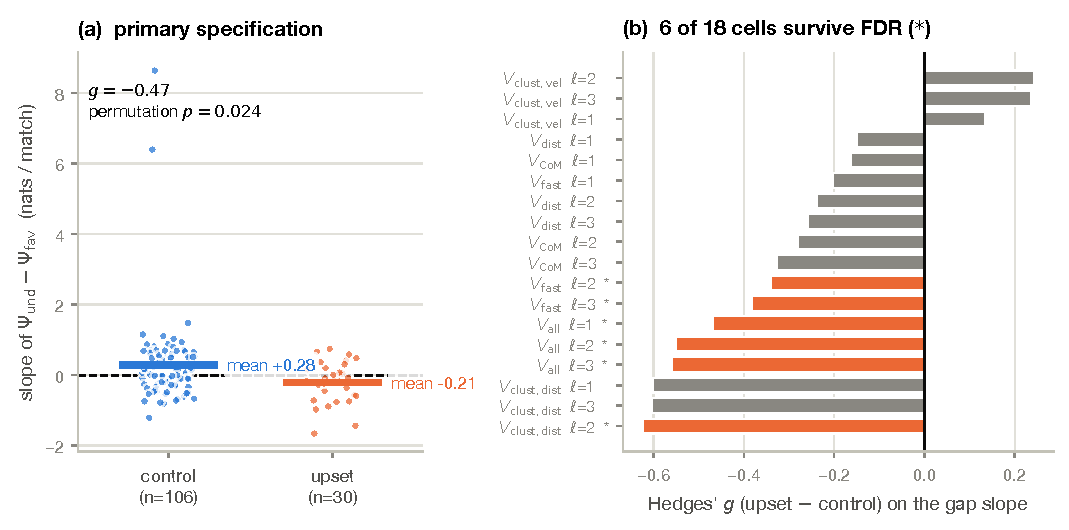
\includegraphics[width=\textwidth]{figures/fig3_gap_trend.pdf}
\caption{The emergence gap trends down in upsets and up in controls.
(a) Per-match least-squares slope of $g(t)=\Psi_{\text{und}}(t)-\Psi_{\text{fav}}(t)$ for
the primary specification (\code{V\_all}, $\ell=1$), horizontal bars are group means.
(b) Hedges' $g$ for the upset--control slope difference in each of the 18 feature $\times$
order cells, starred cells survive FDR correction. $\Vcv$ is the only feature with the
opposite sign, and is not significant in any cell.}
\label{fig:gap}
\end{figure}

\begin{figure}[H]
\centering
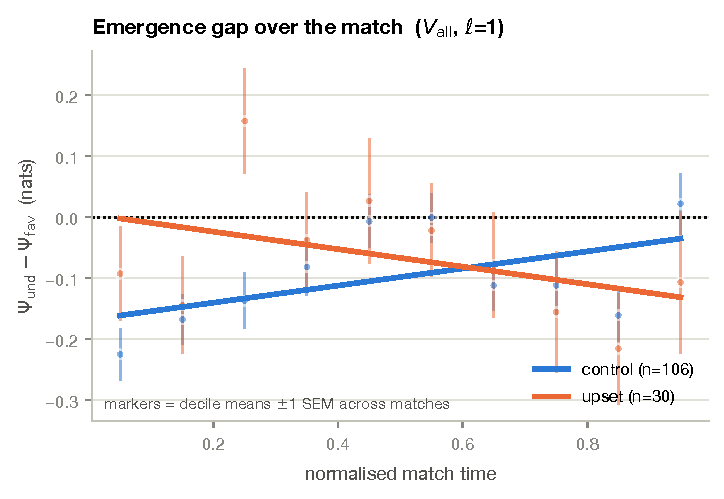
\includegraphics[width=0.6\textwidth]{figures/fig4_gap_trajectory.pdf}
\caption{The same effect as a trajectory. Decile means of the emergence gap over
normalised match time, $\pm1$ SEM across matches, with the fitted trend for each group.
The two groups start indistinguishable and diverge. Note that the mean-curve comparison
itself is \emph{not} significant (\cref{sec:res-rq3}), the tested quantity is the
distribution of per-match slopes shown in \cref{fig:gap}, not the difference between these
two curves.}
\label{fig:traj}
\end{figure}

\paragraph{Interpretation.} More negative $\Psi$ is redundancy-dominated, which
\cite{rosas2020,cheng2025} gloss as synchronised, well-drilled, structured play. A downward
gap slope in upsets means that the underdog becomes progressively more drilled
relative to the favourite as the match develops, while in controls the reverse holds. The downward slope is a trajectory, not a static level, which is why
\cref{sec:res-rq1} missed it. Its direction is opposite to the RQ1 expectation that
underdogs would display higher, positive emergence.

\paragraph{Robustness.} Two control matches have visibly extreme positive slopes. Removing
them strengthens the result ($g=-0.67$, $p=0.0064$), winsorising at the 5th/95th
percentiles also strengthens it ($g=-0.62$, $p=0.0049$), a permutation test on the median
difference gives $p=0.012$. Group medians ($-0.128$ upset, $+0.201$ control) carry the same
sign as the means, and the primary test is based on rank so the effect is not an artefact of
tail behaviour.

\paragraph{Caveats.} This family was examined after the pre-specified tests returned null,
so it is exploratory and requires out-of-sample confirmation. $\Vcv$ shows the opposite
(non-significant) sign in all three orders, so the effect is not uniform across macro
features. Because the $\ell=2$ and $\ell=3$ cells are near-deterministic rescalings of
$\ell=1$ within a feature, ``6 of 18'' overstates the number of independent replications so the effective count is closer to three, one per feature family.

\subsection{RQ4 --- no measurable disruption}
\label{sec:res-rq4}

The proposal specified three conditions: favourite wins; favourite loses to the underdog;
favourite loses to an equally strong opponent. The third does not exist in this
dataset (\cref{sec:corpus}). A general losing effect therefore cannot be separated from a
giant-killing specific one. This is a design limitation, not an analysis choice, and it
means RQ4 as posed is unanswerable with these data.

On the two available conditions, neither the favourite's $\Psi$ (smallest $p=0.263$,
$\Vcv$) nor the disruption coefficient $\mathrm{dc}_{ic}$ (smallest $p=0.397$) differs by
outcome, nothing survives correction. Cross-team coupling is high and near-identical
between groups ($\mathrm{dc}_{ic}\approx0.92$), which is consistent with both teams
tracking the same ball and suggests $\mathrm{dc}_{ic}$ is measuring the shared ball
trajectory rather than tactical disruption.

\subsection{RQ5 --- classification at chance}

Each match contributes seven summary statistics per (macro feature
$\times$ order $\times$ role) trajectory plus EAI and DC summaries: 260 features for 136
matches, a feature-to-observation ratio of $1.9$ which is what the overfitting regime the
design anticipated. Under stratified 5-fold cross-validation the random forest achieves
ROC-AUC $0.547$ and PR-AUC $0.279$ against a base rate of $0.221$; the permutation null,
in which the entire pipeline is re-run on 200 label shuffles, has mean $0.490$ and standard
deviation $0.083$, giving $p=0.255$ (\cref{fig:clf}a). Out-of-time performance under
temporal blocking is unstable across split points ($0.71$, $0.60$, $0.54$ as the training
window grows), which with 7--12 upsets per test block is sampling noise, not evidence of a
usable model.

\paragraph{Feature importance.} Standard per-feature permutation importance
returns exactly zero for all 260 predictors. This is the
consequence of extreme redundancy among near-duplicate columns
(\code{psi\_l1\_mean} versus \code{psi\_l1\_median} on the same trajectory), so permuting
one leaves the forest able to reconstruct it from its neighbours. Importance is therefore
computed out-of-fold, the drop in cross-validated AUC, with permutation applied to
held-out rows only, and grouped, with all 50 columns belonging to one macro feature
permuted together, which is also the form in which RQ5 poses the question
(\cref{fig:clf}b).

Only $\Vcd$ ($+0.036$) and \code{V\_all} ($+0.027$) have positive importance, both within
roughly $1.5$ standard deviations of zero, and four blocks have negative importance, permuting them improves out-of-fold AUC, which is what the noise looks like. Since the
underlying model does not generalise, no block should be described as discriminating giant
killings. RQ5 has no answer beyond none at this sample size. %'' none of them at this sample size'

\begin{figure}[H]
\centering
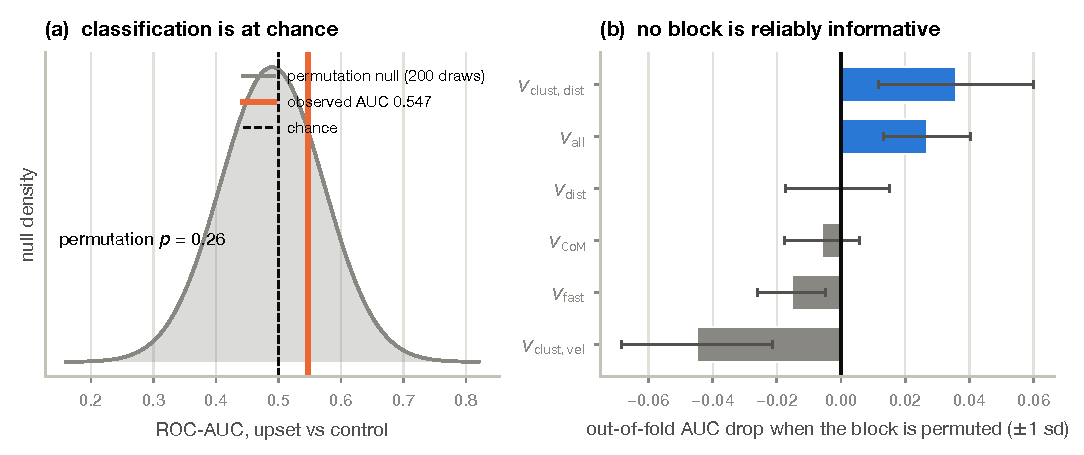
\includegraphics[width=\textwidth]{figures/fig5_classification.pdf}
\caption{\textbf{RQ5 is at chance.} (a) Observed cross-validated ROC-AUC against the
200-draw permutation null (drawn as a normal approximation with the null's mean and
standard deviation). (b) Grouped out-of-fold importance: the AUC drop when all 50 columns
of one macro-feature block are permuted together, $\pm1$ sd across folds. Four of six
blocks have negative importance.}
\label{fig:clf}
\end{figure}

\subsection{Sensitivity}
\label{sec:res-sens}

\paragraph{Specification curve.} An earlier informal pass appeared to find $p<0.05$
effects and used the median as the within-match summary of $\Psi$. Nothing in the
data justifies that over the mean, with skewness $0.03$, excess kurtosis $-0.03$ and yet on identical data we have median $p=0.020$, $10\,\%$ trimmed mean $p=0.058$,
mean $p=0.120$. Rather than choose, we enumerate all 324 combinations
(\cref{fig:sens}a). Median-based specifications clear $p<0.05$ about twice as often as
mean-based ones ($30.6\,\%$ versus $14.8\,\%$) so that single choice does real work, since mean and trimmed-mean specifications supply over half the
significant cells. 323 of 324 specifications give $g<0$ and the single
exception is $+0.00003$. The direction is effectively unanimous even where the magnitude is
not significant.

\paragraph{Placebo calibration.} Repeating the entire specification curve on 25 label
shuffles gives a placebo mean of $3.6\,\%$ of cells at $p<0.05$ (sd $8.5\,\%$) against the
observed $21.9\,\%$, an empirical $p=0.080$ (\cref{fig:sens}b). The real labels produce
roughly six times the placebo rate. We read this as weak evidence for a small real
effect, while noting it does not license any single
specification as a headline.

\paragraph{Definition, outliers, window and $k$.} The upset coefficient is small and
non-significant under every variant of the upset definition (rank gap $\ge0,10,20,30$),
after dropping MAD-flagged outliers, after requiring $n_{\text{eff}}\ge40$, and after
excluding the first and last $10\,\%$ of each match. Recomputing $\Psi$ from scratch at
$W\in\{30,60,90\}$\,s and $k\in\{3,4,7,10\}$ on a 60-match subsample shifts $|\Psi|$
substantially, as expected, but leaves the \code{V\_all} upset effect near zero throughout.
Notably, the $\Vcv$ standardised effect is stable between $-0.48$ and $-0.72$ across every
$W$ and $k$, and reaches nominal significance at $W=90$ ($p=0.027$) and at $k=10$
($p=0.032$) which is consistent with a small, real, consistently-signed effect on the one
non-linear macro feature, and consistent with the reading that longer windows relieve the
saturation of \cref{sec:res-measure}.

\paragraph{Power.} The dataset resolves only $|g|\gtrsim0.58$ at $80\,\%$ power
(\cref{fig:sens}c). Power at $g=0.3$ is $0.31$; at $g=0.5$ it is $0.68$. The proposal asked
for 50--75 matches per group; the upset arm delivered 30. Reaching $80\,\%$ power at
$g=0.3$ against 106 controls would require roughly 150 upsets.

\begin{figure}[H]
\centering
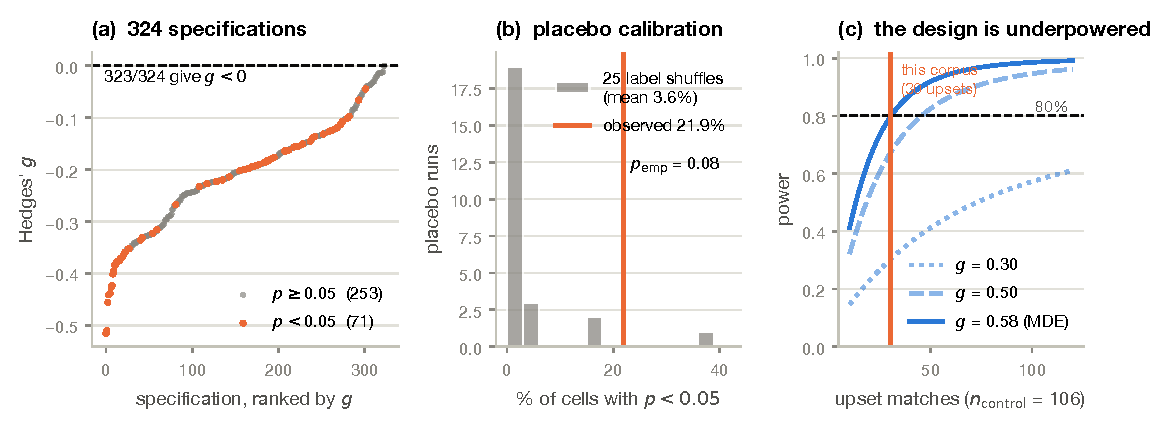
\includegraphics[width=\textwidth]{figures/fig6_sensitivity.pdf}
\caption{\textbf{Sensitivity.} (a) Specification curve: 324 analytic specifications ranked
by effect size; $323$ give $g<0$. (b) Placebo calibration: the observed rate of $p<0.05$
cells against 25 label shuffles of the same curve. (c) Power against the number of upset
matches, holding controls at 106, for three effect sizes.}
\label{fig:sens}
\end{figure}

\subsection{Summary of results}

\begin{table}[H]
\centering
\small
\begin{tabular}{@{}llll@{}}
\toprule
RQ & Question & Tests & Verdict \\
\midrule
RQ1 & emergence signatures & 54 & no effect detected \\
RQ2 & order of emergence & 7 & order profile does not differ by outcome \\
RQ3.a & levels, tipping point & 17 & no tipping point; curves indistinguishable \\
RQ3.b & gap trend & 18 & effect detected ($g=-0.47$, perm.\ $p=0.024$) \\
RQ4 & disruption of favourite & 12 & no effect; third condition unavailable by design \\
RQ5 & classification & 1 & chance (AUC $0.547$, $p=0.26$) \\
\bottomrule
\end{tabular}
\caption{All research questions proposed. RQ3.b was analyzed after the prespecified tests returned
null and is exploratory.}
\label{tab:summary}
\end{table}

% ===========================================================================
\section{Discussion}
\label{sec:discussion}
% ===========================================================================

%\subsection{What the evidence supports}

The level of $\Psi$ does not distinguish giant killings from expected results at any
interaction order, for any macro feature, and under any sensitivity variant. It does not
support classification above chance. The one live result shows that temporally the
underdog-minus-favourite emergence gap drifts downward during upsets and upward during
controls, replicating across six feature--order cells after FDR correction with medium
effect sizes and confirmed by permutation. Since negative $\Psi$ denotes drilled,
redundancy-dominated play, the reading is that underdogs consolidate structure as a
giant killing game unfolds, while favorites lose structure relatively.

%This is a coherent story, and it is the story the event-data literature tells. 
Underdogs
who win usually concede possession and passing accuracy while producing more clearances, more long
balls and more shots on target which implies a disciplined, compact, direct profile. A team playing
that way should look increasingly redundancy-dominated as it settles into a defensive
block. What our result adds is that the phenomenon is dynamic so it is not that
underdogs who win are more drilled on average, the level tests say that they are
not, but that they become so relative to the favourite over the course of the
match. It also inverts the framing of the original hypothesis. We looked for a surge of
synergy and found a consolidation of structure.

We state that this result is exploratory. It was found after the pre-specified
tests returned null. The effective number of independent replications is closer to three
than six, and one macro feature carries the opposite sign. It is a hypothesis worth
pre-registering, not a finding to build on.

\subsection{Why the nulls are not decisive}

Three reasons, in increasing order of importance.

\paragraph{Power.} Minimum detectable effect is $|g|\approx0.58$ against an upset arm of 30.
An effect of $g=0.3$ is perfectly plausible for a construct this indirect but would be
detected here about one time in three. Two pieces of evidence suggest a small real effect
rather than pure noise which are the near-unanimity of sign across 324 specifications, and a
placebo-calibrated excess of significant cells at $p_{\text{emp}}=0.08$. Both point the same way and neither is conclusive.

\paragraph{Definitional redundancy.} Most of what $\Psi$ records here is arithmetic common
to every team in every match. $\Vcom$ is the mean of the micro positions, so every player
is mechanically informative about it, and the whole-minus-sum form then double-counts that
redundancy ten times over. Consistently, the largest standardized effects across the entire
study sit on $\Vcv$, the one macro feature that is not an average of its micro inputs, in RQ1 ($-0.43$), in the window/$k$ sensitivity ($-0.48$ to $-0.72$, stable across
every setting), and in the RQ5 importance ranking, where the two non-linear features are
the only ones with a positive-signed contribution. That pattern is what one would expect if
a small real signal existed and were being masked by definitional redundancy wherever the
macro feature is a linear aggregate.

\paragraph{The criterion cannot express the hypothesis.} This is the substantive point,
and \cref{tab:headroom} makes it precisely. On the four macro features that carry the bulk
of the analysis by magnitude, all of them linear aggregates of the micro state, $\Psi>0$ occurs in $0.004\,\%$ of windows and match-level SRR is zero. 
The understanding that underdogs show
positive emergence in bursts has no range in which to be observed there. $24\,\%$
of the constituent mutual-information terms sit at the estimator's finite-sample ceiling,
so roughly a third of the $\Psi$ values on those features are pinned at a saturation
floor and carry no information about the teams at all. A whole-minus-sum statistic
estimated on 59 samples is the wrong instrument for detecting synergy in a system where
redundancy is this dominant.

The corollary is constructive rather than merely deflationary. The two clustering
coefficients do have positive range, a quarter of $\Vcv$ windows are
synergy-dominated, and they are also where every near-significant effect in this study
sits. The evidence points to real indicators being visible on non-linear
macro features and invisible on linear ones, which is a testable claim and a concrete
design prescription for the next study. We would not now interpret the RQ1 null as
evidence that giant killings lack emergent coordination; we would interpret it as evidence
that this measurement, on these features, cannot see it either way.

\subsection{Relation to prior work}

Cheng et al.\ \cite{cheng2025} report strong, clean correlations between causal emergence
and possession on the same macro features. Why do we see so much less? Three differences,
any of which could be decisive. (i) Data quality. Their tracking is complete 25\,Hz
optical data while ours is reconstructed from sparse freeze frames with a reported off-camera
error of $7.33$\,m \cite{penn2023}. That error is symmetric and averages out for linear
aggregates, but the clustering coefficients are non-linear in the pairwise distances, and
those are precisely the features on which we see the largest standardised effects and the
least redundancy. (ii) Comparison structure. They compare phases and roles
within matches, where the definitional-redundancy floor is common to both sides of
the comparison and cancels. We compare across matches, where it does not, and where
98--99\,\% of the variance is within-match noise. (iii) Estimator. They use a
Gaussian plugin while we use KSG. The Gaussian estimator has no finite-sample ceiling of the
kind documented in \cref{sec:res-measure} and will not saturate. The non-parametric choice
was made to weaken an assumption at the cost of a dynamic-range problem we
did not anticipate.

None of this contradicts \cite{cheng2025}. It does suggest that the within-match results
there do not straightforwardly transfer to between-match outcome prediction, and that the
transfer requires both better tracking and a synergy measure that does not double-count
redundancy.

\subsection{Practical implications}

From a study whose primary results are
null and whose one positive result is exploratory, we may be reluctant to advise tactics for coaches, however three things can be said honestly, 
A fuller statement for practitioners accompanies the
replication package.

First, there is no evidence for the intuition that upsets are produced by a surge of
improvised collective creativity. If it exists, it is smaller than $g\approx0.58$ or
invisible to this measure. The practical implication is negative and worth stating: a coach
should not expect a measurable ``togetherness'' spike to be the mechanism.

Second, the one signal we do see points the other way, toward consolidation.
The underdogs who win look, relative to their opponents, increasingly synchronised and
predictable as the match goes on. If that survives replication, the actionable form is
about trajectory management rather than intensity. The question for an underdog is
not how coordinated the team is at kick-off but whether its structure holds and tightens
as the match progresses, when fatigue and score pressure act against it. That is
trainable in a way ``wanting it more'' is not.

Third, structure appears to matter more than movement synchrony. Every part of this
study where anything approached significance involved a spatial-configuration feature,
inverse-distance clustering, or the joint feature containing it, and $\Vcv$, velocity
similarity, is the one feature that consistently either shows nothing or points the other
way. This echoes \cite{cheng2025}, who found velocity-similarity clustering uncorrelated
with possession while positional features correlated strongly. Compactness and spacing
appear to be where team-level information lives while running in the same direction at the same
time does not appear to be.

%%%%%%%
\subsection{Limitations}

\begin{enumerate}
\item Sample. 30 upsets against a target of 50--75. Every inferential conclusion
in this paper is secondary to $n$.
\item Reconstructed tracking. $7.33$\,m mean off-camera error, uncalibrated against
the Everett et al.\ \cite{everett2023} imputer. The non-linear clustering features are the
most exposed to this and are also where the largest effects sit.
\item Dataset composition. Eight competition-seasons, overwhelmingly international
tournaments. Cup competitions, where giant killings are most common and most culturally
salient, are absent.
\item No even-game stratum RQ4 is unanswerable by design.
\item Estimator saturation. Roughly a third of window-level $\Psi$ values are at
a floor imposed by the estimator's dynamic range at $N\approx59$.
\item Exploratory positive result. RQ3b was not pre-specified.
\item Analytic degrees of freedom. The within-match summary statistic alone moves
$p$ from $0.02$ to $0.12$ on identical data. We report the full specification curve rather
than a choice, but the fact remains that this literature can produce either answer.
\end{enumerate}

\subsection{Recommendations}

\begin{enumerate}
\item Confirm the gap-trend effect out of sample. Pre-register the slope of the
underdog--favourite gap as the primary endpoint, with \code{V\_all} at $\ell=1$ and the mean
as the within-match summary, and test on held-out matches. This is the single highest-value
next step.
\item Replace whole-minus-sum $\Psi$ with the $\Phi$ID-based synergy of Rosas et
al.\ \S III\,B \cite{rosas2020,mediano2021}, which does not double-count redundancy across
marginals and can therefore represent positive emergence. This addresses the deepest
problem identified here.
\item Lengthen the window to $W=90$--$120$\,s, or increase $k$, to lift the
estimator ceiling. The $\Vcv$ effect reaches nominal significance at $W=90$ and $k=10$,
which is what one expects if saturation is masking signal.
\item Prefer non-linear macro features $\Vcv$ and $\Vcd$ have the lowest
definitional-redundancy floor and carry the largest standardised effects.
\item Expand the upset arm toward 150 matches, drawing on cup competitions, and
add an even-match loss stratum so RQ4 becomes answerable.
\item Cross-validate the tracking reconstruction against the LSTM--GNN imputer
of \cite{everett2023} before interpreting any clustering-coefficient result.
\end{enumerate}

% ===========================================================================
\section{Conclusion}
% ===========================================================================

We set out to test whether giant killings carry an information-theoretic signature of
emergent coordination. On the level of the causal-emergence coefficient $\Psi$, they do
not. Of the 54 pre-specified tests, three interaction orders, six macro features, a full
sensitivity battery and a classifier all return null values. One exploratory result that is significant is the underdog-minus-favourite emergence gap trends downward over the match in upsets and
upward in controls which points toward consolidation of structure rather than a surge
of synergy.

The more transferable finding is about the instrument. On 60-second windows of football
tracking data, $\Psi$ correlates at $r=0.9996$ with the negated micro sum and is pinned at
an estimator-imposed floor over roughly a third of its range. It is dominated by the
arithmetic fact that a team's centre of mass is the mean of its players' positions --- and
that domination is specific: on macro features that are linear aggregates of the micro
state, $\Psi$ is positive in $0.004\,\%$ of windows and the criterion has no usable range;
on the clustering coefficients, which are not, it is positive up to a quarter of the time.
Researchers applying causal emergence to team sports should expect this and design around
it: use synergy measures that do not double-count redundancy, prefer macro features that
are not linear aggregates of the micro state, and check the estimator's dynamic range
before interpreting a negative result. The question of whether giant killings are emergent
remains open. It is open for better reasons now than when we started.

% ===========================================================================
\section*{Data and code availability}
% ===========================================================================

All code, processed data, figures and result tables are in the replication package
accompanying this manuscript. Source data are StatsBomb open data \cite{statsbomb},
FBref, Transfermarkt and Understat, all publicly available and used in accordance with
their terms. No personally identifiable information is used; tracking data are aggregated
to team-level features. Raw provider data are not redistributed; the pipeline reproduces
them from public sources.

\section*{Ethics}

This study analyses publicly available match data on professional athletes acting in a
public professional capacity. No human-subjects approval was required.

\bibliographystyle{plain}
\bibliography{refs}

% ===========================================================================
\appendix
\section{Output schema}
% ===========================================================================

\code{data/caus\_emg/\{match\_id\}\_caus.\{csv,parquet\}} --- one row per (match, team,
window, macro feature); 63 columns.

\begin{table}[H]
\centering
\small
\begin{tabular}{@{}lp{9.6cm}@{}}
\toprule
\textbf{Group} & \textbf{Columns} \\
\midrule
Identity      & \code{match\_id, outcome, competition, team, opponent, role, team\_rank} \\
Window        & \code{window\_start, t\_abs, minute, macro\_feature, n\_eff, frac\_valid} \\
Information   & \code{I\_macro, H\_macro, I\_micro\_l1..3, I\_micro\_l1c} \\
$\Psi$        & \code{psi\_l1, psi\_l2, psi\_l3, psi\_l3\_raw, psi\_l1c} \\
Subset counts & \code{n\_terms\_l1..3, n\_total\_l1..3} \\
EAI           & \code{eai\_l1..3, eai\_stab\_l1..3, eai\_denom\_l1} \\
DC            & \code{i\_cross, h\_fav, h\_und, dc, dc\_rev, dc\_ic} \\
SRR           & \code{srr\_l1..3, srr\_roll\_l1..3, srr\_match\_l1..3} \\
Diagnostics   & \code{estimate\_ok, neg\_mi\_flag, mono\_violation, psi\_l1\_z, is\_outlier, eai\_unstable, dc\_unstable} \\
\bottomrule
\end{tabular}
\end{table}

\section{Diagnostic counts from the production run}

\begin{table}[H]
\centering
\small
\begin{tabular}{@{}lr@{}}
\toprule
Matches processed                      & 136 (all \code{ok}) \\
Window-level records                   & $1{,}384{,}566$ \\
Distinct windows                       & $116{,}709$ \\
Estimates successfully computed        & $99.98\,\%$ \\
Median usable frames per window        & 59 of 59 \\
Reconciliation error against Sprint 3  & $0.0$ nats over $9{,}371$ windows \\
Compute                                & $4{,}898$ core-minutes \\
\midrule
Flagged: MAD outliers                  & $6{,}049$ \\
Flagged: negative $I_{\text{macro}}$   & $4{,}255$ \\
Flagged: order-monotonicity violations & $55{,}594$ \\
Flagged: unstable EAI denominator      & $58$ \\
Flagged: unstable DC denominator       & $147{,}456$ \\
\bottomrule
\end{tabular}
\end{table}

The large DC flag count is the differential-entropy problem of \cref{sec:metrics} doing its
job: $|H(V_f)|<1$ nat for the low-variance clustering features, so the literal ratio is
uninterpretable there and $\mathrm{dc}_{ic}$ should be used instead.

\end{document}
